\chapter{系統架構與方法}
\label{chapter:system}



\section{系統架構}
\label{sec:systemarchi}
本研究專注於透過設計資料庫並用其資料訓練夾取可行性預測系統,並以此作為線索作為雙手臂主動式操作系統的策略因此可分為三大部分:商品語意基準資料庫、夾取可行性預測系統、雙手臂主動式操作系統。基準資料庫目的在設計一個專門給日常商品的資料庫,此資料庫包含物品場景圖片、商品語意如商品整體遮罩、條碼遮罩、品牌文字遮罩,因此可利用這份資料集訓練夾取可行性預測系統,基準資料庫包含參考Amazon Picking Challenge來選取物品、實驗環境設計、並分別搭建現實與虛擬環境以蒐集資料並加以驗證。而夾取可行性預測系統則是改善~\cite{peterthesis}所提出之商品文字姿態估計系統之缺點,並改良成雙手臂夾取可行性預測系統,此系統包含品牌文字、物品語意分割、以及基於語意與三維點雲資訊之夾取可行性預測。而最後的雙手臂主動式操作系統則是設計雙手臂協作方式、手臂功能、假爪選擇與設計、以及最後執行任務之有限狀態機(Finite State Machine)。此系統的設計考量與基準資料庫物品選擇、夾取可行性預測系統環環相扣,因此接下來將先說明環境架設以及主動式操作系統硬體設計,接下來依序說明如何蒐集商品語意基準資料庫、夾取可行性預測系統。最後以主動式操作系統有限狀態機總結整體系統。

\section{硬體架構與工作環境配置}
本研究提出的系統建立在兩隻協作型手臂上。一為協作手臂UR5,並裝上Robotiq 2F-85雙指假爪作為末端效應器以及RGB-D深度攝影機Realsense SR300,另一隻手臂則是則是UR3,並裝上自製的吸盤假爪。這兩隻手臂被固定在同一張桌上,並彼此距離1公尺。此外,桌上有兩個盒子在手臂之間,一個盒子是被裝滿物品的,而另一個而是空的。裝滿物體的盒子上有配置深度攝影機,作為觀察盒子物體用。整個系統會從充滿物品的盒子開始:UR3把物體從雜亂的盒子中取出,並放到空盒或停留於空中作為暫時位置,等待UR5夾取並以特定姿勢擺放至架上固定的格子裡。

\begin{figure}[ht]
	\centering
	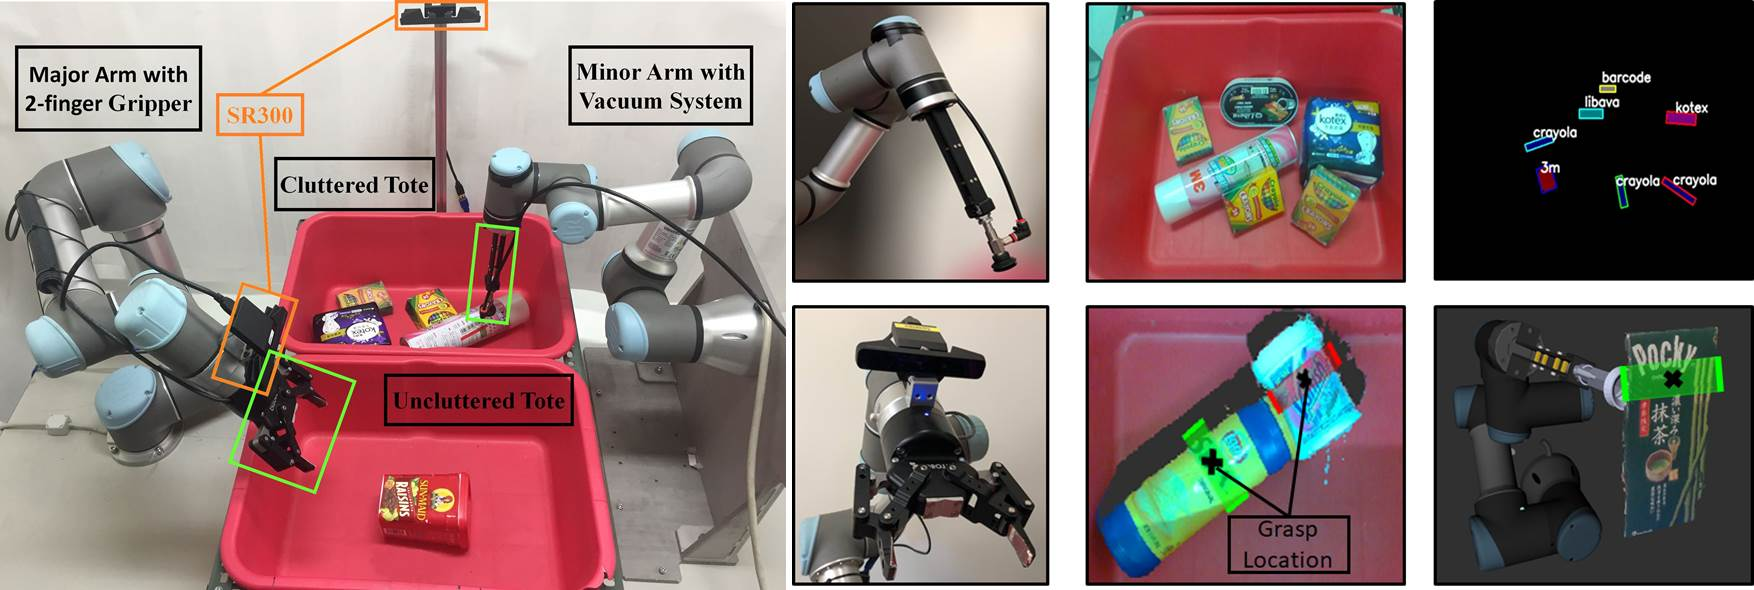
\includegraphics[height=!, width=1.0\linewidth, keepaspectratio=true]
	{./figures/hardware_archi.jpg}
  \caption{圖1.左圖:本研究提出雙手臂主動式操作系統去主動改變場景以達到改善機器人感知環境能力,並最佳化物品夾取可行性系統的效果。吸盤假爪從一個雜亂環境移動物品去取得被隱蔽或部分遮蔽的品牌文字資訊。而雙指假爪則藉由基於品牌文字之線索預測夾取點,以此去完成特定姿態的物品擺放任務。右圖:基於品牌文字,本研究可在雜亂環境中預測品牌文字姿態,並以此針對吸盤假爪與雙指假爪進行物品夾取可能性預測。}
  \label{figure:hardware_archi}
\end{figure}


\subsection{設備介紹}
本研究專注於機器人主動式操作系統,因此手臂、假爪、感測器之選擇十分重要,因此將會逐一分析使用設備之性能以及使用原因。

\paragraph{UR5與UR3協作式機械手臂}
UR5與UR3協作機械手臂乃優傲機械人有限公司(Universal Robots)所生產之協做式機器人,乃六軸機械手臂,其特點為可支援機器人作業系統(Robotic Operation System),適合研究人員快速開發,並擁有安全機制,任意軸碰撞到人或物體,便會自動停止。此外精度都可達至0.1mm,且每軸最快速度可以達到每秒180/360度。UR3/5的活動空間為半徑0.5/0.85m,而承重則分別是3/5 KG,因此本研究所夾取之物品皆低於3公斤以內。考量研究與未來應用之安全性、活動空間以及易開發性,本研究選擇UR5與UR3作為手臂使用。

\begin{figure}[ht]
	\centering
	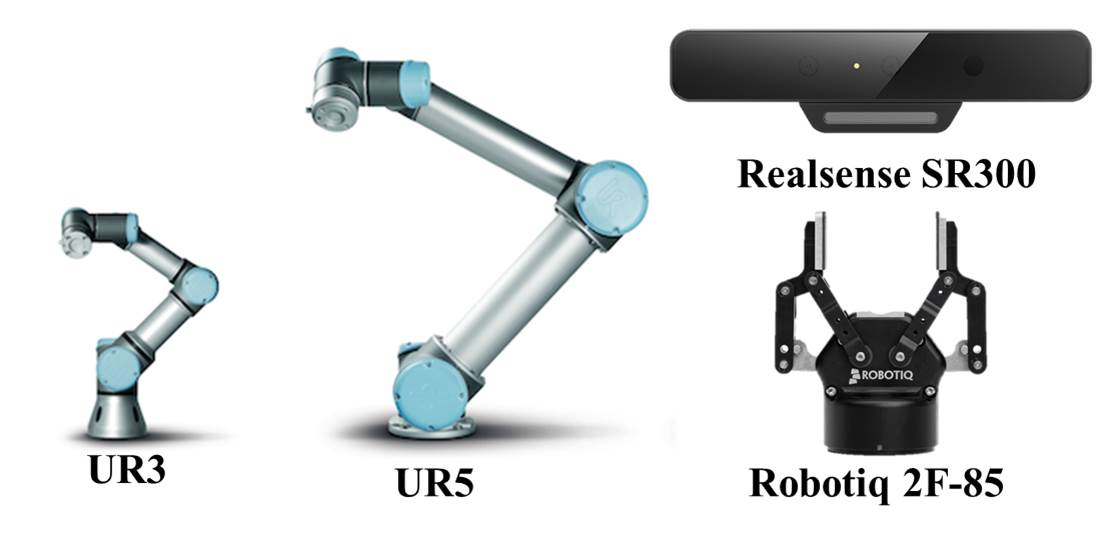
\includegraphics[height=!, width=1.0\linewidth, keepaspectratio=true]
	{./figures/hardware_list.jpg}
  \caption{本研究使用之感測器、機械手臂、假爪。}
  \label{figure:hardware_list}
\end{figure}

\paragraph{Robotiq 2F-85 假爪}
Robotiq 2F-85假爪為機器人公司Robotiq所研發,專門用於機械手臂上的2指假爪。其特色在於其假爪兩指是平行的。並非像人一般是多指靈巧手,雖然變化性較低,卻十分用來夾取形狀簡單的物品。此外此假爪夾取力道可控制從20牛頓至235牛頓,可穩定夾取物品,且重量只有0.9 公斤,並可以裝於UR5末端。它也支援本研究之平台ROS,因此本研究選擇此假爪裝於UR5上,並執行最後特定姿勢的物件夾取與放置任務。

\paragraph{自製吸盤假爪系統}
此系統乃本研究為主動式操作系統特別開發。此系統包含空氣壓縮機、真空產生器、吸盤假爪、以及控制板Arduino UNO。空氣壓縮機乃使用SWAN空氣壓縮機公司之DRS-210-39無油式空壓機,使用壓力可達7 kg/$cm^{2}$,並儲存39公升空氣。而真空產生器則採用MISUMI公司之VJHB6-7,產出之氣壓可達-0.95 kg/$cm^{2}$,且有真空產生、真空破壞等多段式氣壓調整功能。最後搭配自製之吸盤假爪,此吸盤夾爪可裝於UR3上,並補足其工作範圍較小的問題,此外吸盤內徑為0.02cm,搭配真空產生器、空氣壓縮機,垂直作用力可達3 kg,可應付市面上大部分的商品。Arduino UNO作為最簡易的控制開發版,用來控制真空產生器,調整吸盤吸力力道。

\begin{figure}[ht]
	\centering
	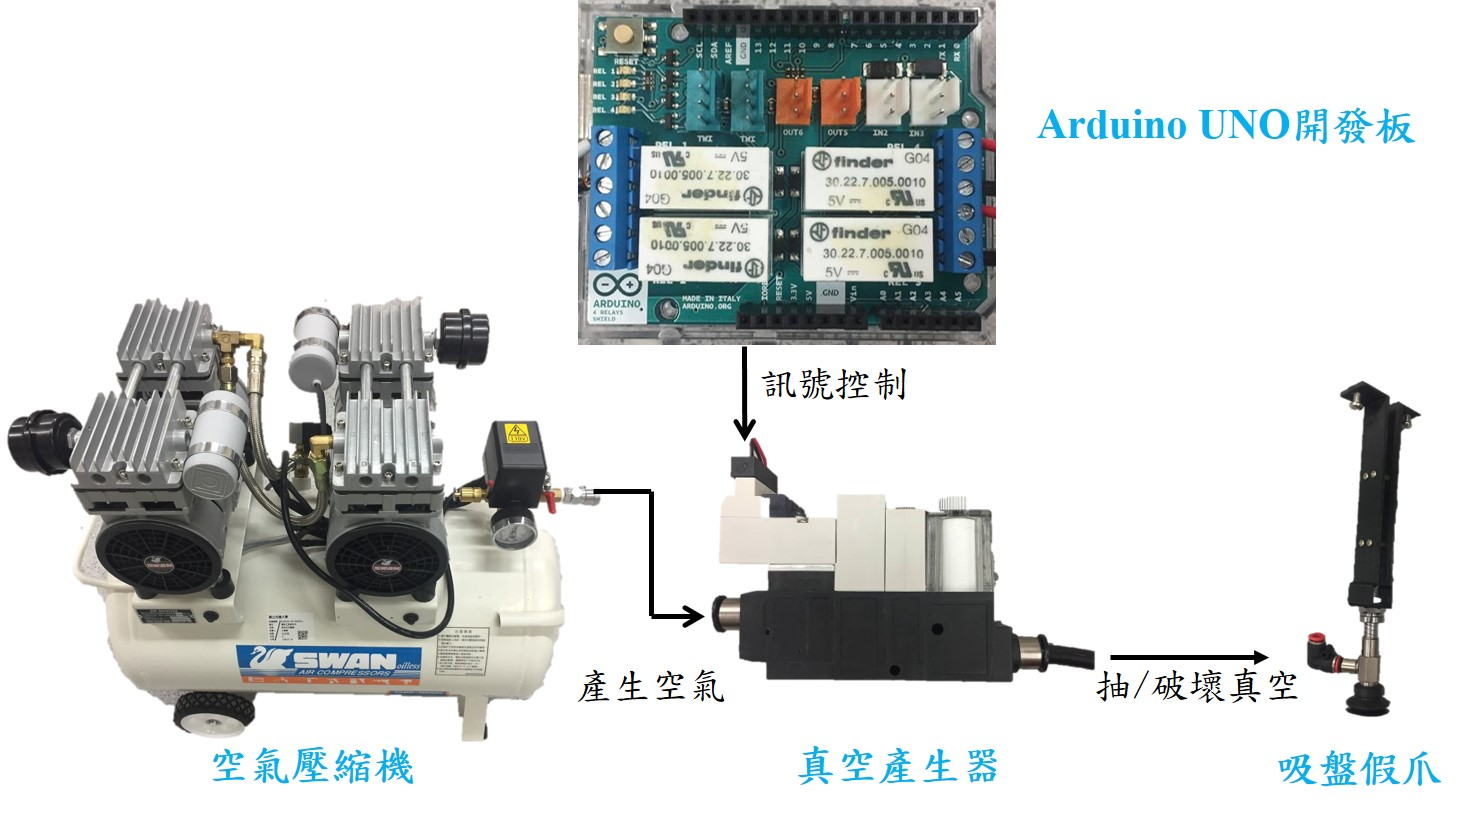
\includegraphics[height=!, width=1.0\linewidth, keepaspectratio=true]
	{./figures/suction_system.jpg}
  \caption{吸盤假爪系統。}
  \label{figure:suction_gripper}
\end{figure}

\paragraph{RGB-D深度攝影機Realsense SR300}
RGB-D 深度攝影機Realsense SR300乃Intel公司所研發,專用於觀察室內近距離場景,其利用紅外線感知深度,同時具有彩色與深度資訊,操作範圍在0.3 - 2m之間,景深為(H: 73, V: 59, D: 90),且影格率(Frame rate)可達30fps。此感測器雖觀察視野不大,卻能得到視野內非常濃密知點雲資訊,十分適合用於觀測物品點雲,姿態預測用,此外此攝影機也有支援ROS,很適合開發者使用。因此本研究選擇將Realsense SR300安裝於UR5與盒子上,用於觀察物品。

\subsection{多視角主動式視覺}
此系統包含兩個深度攝影機Realsense SR300, 一個裝於 UR5 上,用於在於可控制手臂位置以改變視角改善感知能力,讓此系統可以解決品牌文字被遮蔽之狀況,在主動式操作系統主要用來觀察被夾取至空間並停留或是背放置空盒的物體。而另一個 SR300 則裝於桌上並面對充滿雜亂物品的盒子。此感測器專門用來觀察處在雜亂環境的物品。

\subsection{手臂假爪配置}
本研究目標為將物品以特定姿態夾取與擺放至架上,考慮物品在雜亂環境中難以一次性以特定姿態去夾取並放置,因此設計不同的假爪給不同的手臂與2階段主動式操作系統:吸盤假爪(UR3)用於第一次夾取,從雜亂環境中夾取至空曠環境,而雙指假爪(UR5)則進行第二次的特定姿態夾取及放置。這樣的設計考量不同假爪的特性:吸盤假爪由於與物品的接觸空間小,容易夾取但移動時不穩定,因此適合用於雜亂環境中的夾取,而雙指假爪則相反,與物品的接觸空間小,夾取物品須有特定姿態,且容易受物體遮蔽影響,但夾取後移動相對穩定,因此用於第二次的夾取。


\section{商品語意資料庫}
就本研究所知,本研究之商品語意基準資料庫為第一個資料庫專注於使用語意標註進行特定姿態放置。有許多相關聯的研究如以場景為單位的Grocery Dataset ~\cite{jund2016freiburg},此資料集蒐集25類物品並專注於場景中物品的分類,而不是語意切割。以物體為單位之``Shelf \& Tote''資料集,雖也是進行語意標註,但專注於夾取,而不是放置。本研究建立之資料庫包含以物件為單位以及品牌文字、條碼語意為單位之標註,並整理成3大資料集:1. 現實世界訓練資料集:蒐集來自現實,並包含現實環境噪音(亮暗變化、反射)、不同色調的資料。這組訓練集將被用來訓練物品語意切割模型以及品牌文字語意切割模型。2. 虛擬環境訓練資料集:來自虛擬環境Unity,並參考現實世界設定去蒐集。3. 真實世界測試資料集:包含簡單與複雜困難場景,場景中有雜亂、遮頁、複製品狀況發生。這組測試集將被用來比較評估主動式操作與~\cite{peterthesis}之效能。

\subsection{選用物品}
本研究選用之商品參考Amaxon Picking Challenge 2016, 2017年所用之物品,從中挑選一些堅固不容易變形之物品、並加入其餘商品成為最後的20類目標物品。這些商品包含市面上常見的可樂、番茄醬罐、洋芋片等(請參考圖~\ref{figure:20_products}),皆是常被放置於貨架上讓消費者挑選的物品。選用之商品皆符合前段講述之規則。在這20類商品中依照形狀分類可再在分類成8個圓柱體以及12個長方體。

\begin{figure}[ht]
	\centering
	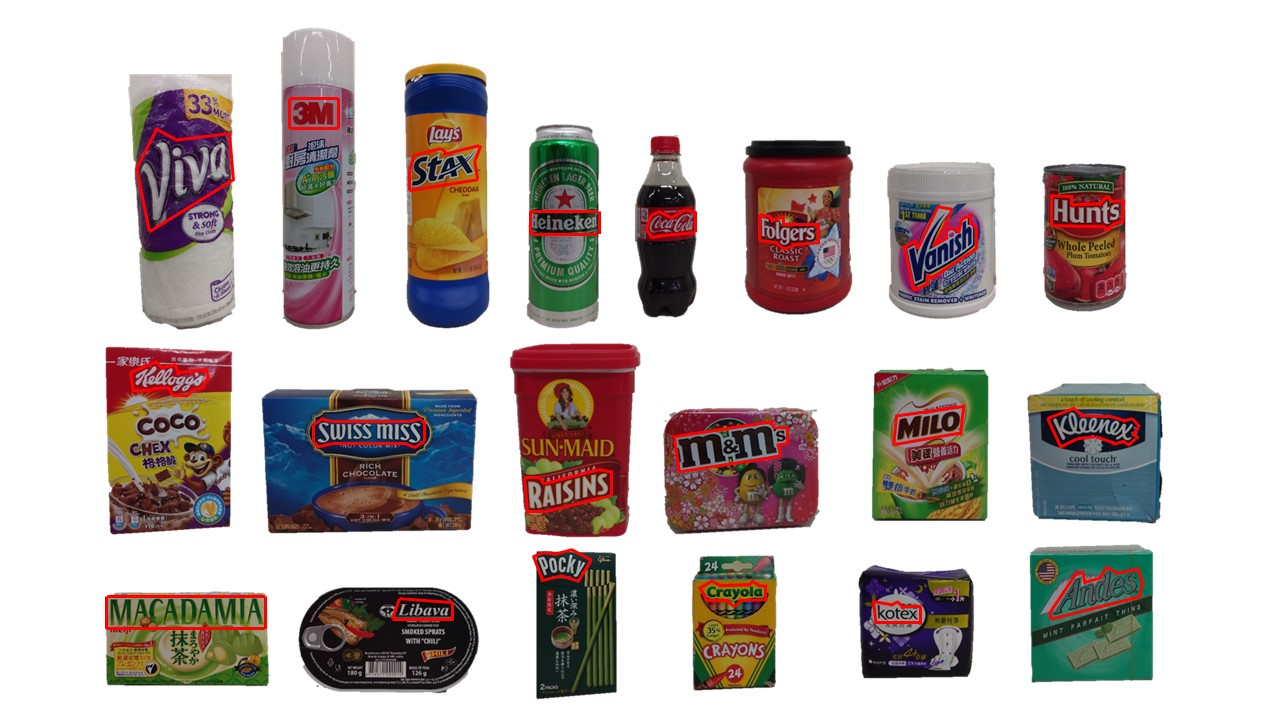
\includegraphics[height=!, width=1.0\linewidth, keepaspectratio=true]
	{./figures/20_products.jpg}
  \caption{20類目標商品及標注示範。}
  \label{figure:20_products}
\end{figure}

\subsection{真實世界訓練集}
這部分資料集蒐集的方法參考這份研究~\cite{zeng2016multi},這份研究的技術也被應用於Amazon Picking Challenge 2016。每一個場景中,單一物品被隨意放置於盒子中,一個RGB-D攝影機安裝於UR5上,用於可系統的移動手臂並在多個視角自動蒐集資料。本研究選擇20個商品做為目標物品,這些物品皆遵守以下的規則:1. 品牌文字高度皆至少大於1.5cm。 2.品牌文字皆為單行。3. 品牌文字不重複出現於物品上。資料集總共有920 scenes $\times$ 31 views。但由於硬體因素,過程中有22張圖片遺漏,因此總共有28,498張圖片。

\paragraph{物體標注}
為了自動化像素級別的物件標註,本研究利用全卷積網路以及影像處理演算法去建造一個半自動資料標註系統。在訓練集中,拍攝下的影像中都只會有惟一的物體放置於盒內,再加上少許的地面,因此背景較單純。利用背景的單純,便可以利用少許的資料訓練出一個2類(物體、背景)的物件切割模型,此模型有能力去分辨背景與物件。為了建立半自動資料標註系統,使用標註工具~\cite{russell2008labelme}先標註約500張圖片。之後運用這些標註資料作為訓練資料對全卷積網路VGG16-FCN權重進行微調後,來對剩餘圖片預測像素級別的物件切割。由於標註資料不多,因此預測結果仍會有一些雜訊,因此取範圍最大的區域作為最後的標註結果。雖然藉由模型來標註的結果不會完全與人為標註相同,但也足夠做為標註資料作為20+1類的物件語意切割模型的訓練資料。

\begin{figure}[ht]
	\centering
	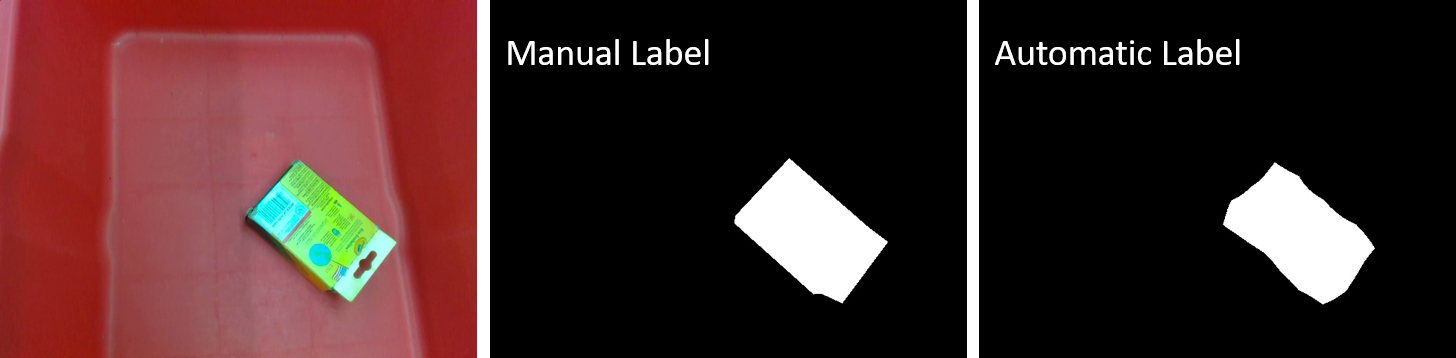
\includegraphics[height=!, width=1.0\linewidth, keepaspectratio=true]
	{./figures/auto_object_label.png}
  \caption{自動標注與人為標註之比較。觀察自動與人為標註之結果,可發現自動標註在邊緣部份效果較不好,與平滑的人為標注相比,多出許多稜角出來。但此結果仍足以作為訓練資料使用。}
  \label{figure:auto_object_label}
\end{figure}


\paragraph{品牌文字標注}
為了訓練一個具旋轉差異性(rotation-variant)且完整無遮蔽的品牌文字偵測器。因此一個本研究設計一個具旋轉差異性的標註規則:當品牌文字方向與水平線夾角介於-45$^{\circ}$ $\sim$ 45$^{\circ}$ 之間,而且品牌文字區域需有一半以上是看的見的,品牌文字才可以被標註。因此在28498張圖片中共有30\%的圖片被標註品牌文字。品牌文字的標註方法是用多邊形框住的。

\paragraph{條型碼標注}
型碼就像是商品的身分證,無論在物流運送、商店結帳、盤貨,都是不可或缺的存在。因此建立商品語意資料庫,條型碼也是重要的標註資料。但條型碼的資料佔的區域較小,因此在在28498張圖片中共有20\%的圖片被標註品牌文字。


\begin{figure}[ht]
	\centering
	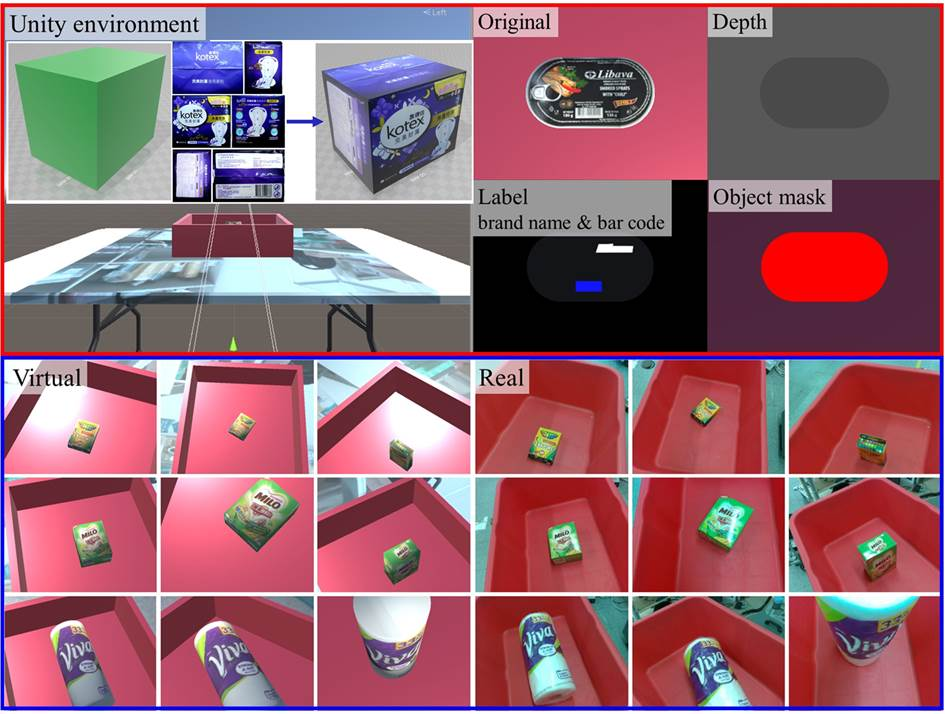
\includegraphics[height=!, width=0.8\linewidth, keepaspectratio=true]
	{./figures/real_and_vir_environment.jpg}
  \caption{於現實與虛擬環境蒐集訓練集。左上:虛擬環境建立示意圖。右上:虛擬資料標注自動標注。藉由3D Builder創造物品三維模型,之後建立相似現實環境的紅色盒子於Unity中,並架設相機與物品以蒐集虛擬資料集。蒐集資料時在虛擬與現實的每一個場景中都只有一個物品,這靈感取自~\cite{}說明在單一場景單一物品並利用巨量資料集的訓練語意切割模型之下,在之後多物品場景的情況下仍能得到不錯效果。}
  \label{figure:benchmark-dataset}
\end{figure}


\subsection{虛擬世界訓練集}
\paragraph{建置虛擬環境}
了建立一個逼真現實世界的虛擬環境,本研究在Unity建立一個相仿真實盒子規格(顏色、尺寸)的模擬盒子,並在蒐集資料時隨機調整虛擬環境亮度(請參考圖~ref{figure:benchmark-dataset}),此外針對物品模型,為了避免三維模型扭曲,與得到高解析度的材質貼圖(texture),本研究使用3D建模軟體3D Builder ~\cite{3DBuilder},手動繪製3D模型,並用高解析度相機近距離所拍攝之物品圖片作為材質貼圖嵌入模型中,成為最後之模型。此外本研究也在模擬環境中加入多顆彩色與深度相機去蒐集虛擬世界中的資料。相機中有些專門拍攝物體、有些則拍攝場景、盒子,藉此讓虛擬環境中的標註資料可自動取得,可大量產生虛擬訓練資料。資料集有200 scenes$\times$ 54 views,共10800張圖片。附註:本研究以10800張虛擬資料作為虛擬資料庫示範用,這些資料可在短時間內大量自動蒐集。


\paragraph{資料增強}
參考蒐集到的真實環境資料可發現,在真實環境中,常有兩大圖片噪音:動態模糊(motion blur)以及失焦高斯噪音(out of focus Gaussian noise),因此本研究將這些干擾加入蒐集好的虛擬資料去增加虛擬資料的變異性。總共加入各自2類的動態模糊與失焦高斯噪音,因此資料量提升至原本的4倍,共43200張圖片。

\begin{table}[ht]
\caption{Numbers of scene, view, and data augmentations carried out in the proposed training sets from real and virtual environments. OBJ (object), BN (brandname), and BAR (barcode) are manually annotated in real set and automatically generated in the virtual set.}
\centering
\begin{tabular}{rrrr|rrr}
\hline
         & Scene & View & Aug. & OBJ       & BN       & BAR \\ \hline
Real Env. 	& 920   & 31   & -        & 28,498       & 8,576    & 5,686     \\
Virtual Env.   	& 200   & 54   & 4      & 43,200       & 24,624         & 14,508          \\
%(Objects)   & 2152  & 15   & 4        & 129,120      & -        & -         \\
\hline
\label{table:training_set_table}
\end{tabular}
\end{table}

\subsection{真實世界測試集}
不同於訓練資料集,在此測試集中,考量手臂假爪範圍與重量限制限制,只選用20類物品中的10類物品做為測試集。此外測試集的場景中同時會出現1 $\sim$ 7個物品,且場景中有物品們相鄰與遮蔽的情況。在此測試集中可再細分為6個子測試集(請參考圖~\ref{figure:testset})。在Single-1, Duplicate-2, and Multiple-2這3個子測試集中,有品牌文字那一面皆是朝上,但在Duplicate-2, and Multiple-2有遮蔽情況發生,所以不一定看的見品牌文字。而其餘3個子測試集Clutter-3, Clutter-5, and Clutter-7則是屬於較複雜的場景,品牌文字隨機朝上或朝下,且遮蔽與堆疊情況更加嚴重。總和真實環境測試集,總共有290個場景、710個物體、476個可視的品牌文字。此外在此測試集中,物體、品牌文字、條型碼都有人員手動標註。

\paragraph{Single-1}
在此子測試集中,每個物品以5個不同的角度被放置,且品牌文字皆朝上,因此總共有5 angle $\times$ 10 objects,共50個場景。此測試集適合用來測試一個操作系統在單一物品但任意旋轉角度、位置情況下, 能否有效進行夾取與放置任務。

\paragraph{Duplicate-2}
在此子測試集中,兩個相同物品被放置於盒內,位置與放置角度也是隨機選擇,因此會出現分開、相鄰、重疊情況發生。共有90個場景。此測試集適合用來測試操作系統在相同物品情況下,是否可以有效切割,進行夾取與放置任務。

\paragraph{Multiple-2}
與Duplicate-2相似,在此測試集中,兩個不同物品被放置於盒內,位置與放置角度也是隨機選擇,並共有90個場景。這個測試集是為了測試操作系統能否應付同時有不同物品在同個場景的情況。

\paragraph{Clutter-3, 5, 7}
在這3個子測試集,遮蔽、雜亂、堆疊情況隨著數量增加而變的更困難與複雜,更趨近於真實環境的上架任務場景。因此非常適合用來評估操作系統能否有效應付噪音、遮蔽、雜亂的問題。


\begin{figure}[htb]
	\centering
	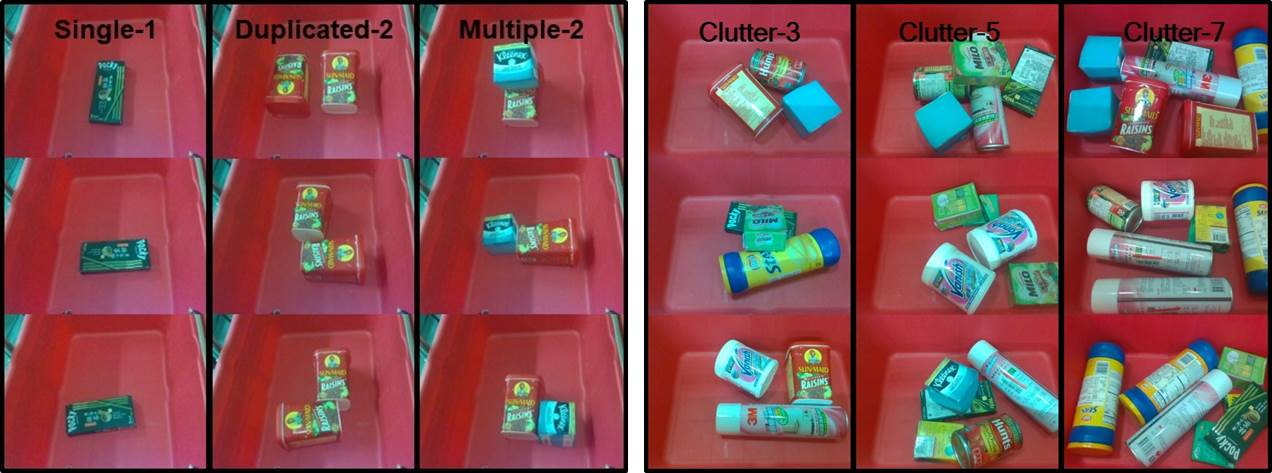
\includegraphics[height=!, width=0.9\linewidth, keepaspectratio=true]
	{./figures/testset.jpg}
  \caption{本研究將測試集分為簡單與複雜場景。在簡單場景中(左)可再細分為Single-1、Duplicated-2、Multiple-2,這3類場景雖會出現相鄰、互相遮蔽情況,但品牌文字皆朝上。而複雜場景中,雜亂程度與遮蔽情況更為明顯,按複雜度分類可再細分為Clutter-3、Clutter-5、Clutter-7,數字代表場景中會出現的物品數量。再這些場景中,物品乃隨意擺置,因此品牌文字可能朝上或朝下看不見。}
  \label{figure:testset}
\end{figure}


\section{基於品牌文字之夾取可行性預測}
本研究之雙手臂主動式操作系統,目的在夾取物品並放置到架子上指定的格子上,並且讓物品排列整齊,且品牌文字朝前,如商店一般。方法乃是藉由夾取可行性地圖為線索,來決定如何使用吸盤假爪夾取物品置空曠空間,並使用雙指夾爪以特定姿態的夾取放置任務。這個而此夾取可行性地圖主要乃是基於具旋轉差異性之品牌文字切割與姿態預測。但在所有品牌文字皆遮蔽的情況下,夾取可行性地圖便會轉為以物品語意與幾何為線索,來生成地圖。

\subsection{品牌文字語意切割與姿態預測}
多發展很久的以物件為單元的物件偵測器可以產生邊界框(Bounding Box)框住物體,這樣的方法不足以去解決考慮特定姿態放置的問題。因此本研究使用品牌文字作為線索去處理物件姿態的問題。這樣的好處是文字以閱讀上來說本身便具有方向性,且文字有其規律性。因此,本研究以品牌文字姿態(文字方向作為X軸、文字平面法向量作為Z軸)去定義物件姿態。並以全卷積網路架構FCN-VGG-DICTNET~\cite{peterthesis}訓練出一個全卷積網路模型,目標去偵測具旋轉差異性的品牌文字。換句話說,本研究預期當品牌文字與圖片水平線夾角介於-45$^{\circ}$ $\sim$ 45$^{\circ}$ 之間,才偵測的出來。如此藉由旋轉圖片4次(0$^{\circ}$、90$^{\circ}$、180$^{\circ}$、270$^{\circ}$)方式再進行預測,預訓練模型可達到在任何角度都能找到具旋轉差異性的遮罩。之後由於在一個場景中可能有多個品牌文字,利用Seed filling algorithm找到連結在一起的同一類,並視為一個品牌文字遮罩。此外在文字角度接近45$^{\circ}$、-45$^{\circ}$可能會在不同旋轉角度圖片都預測出相同的品牌文字,這種情況下,本研究選擇較大的遮罩並不考慮較小的遮罩。以上是關於考慮旋轉差異性的品牌文字遮罩生成方法,接下來將討論如何生成文字姿態。基於選用之品牌文字皆為單行,因此可假設遮罩為一個旋轉矩形,並找出長邊作為文字方向,利用此遮罩與點雲的結合,以此使用品牌文字姿態的定義(文字方向作為X軸、文字平面法向量作為Z軸)進行計算(請參考圖~\ref{figure:text-pose-extimation-pipeline})。

\begin{figure}[ht]
	\centering
	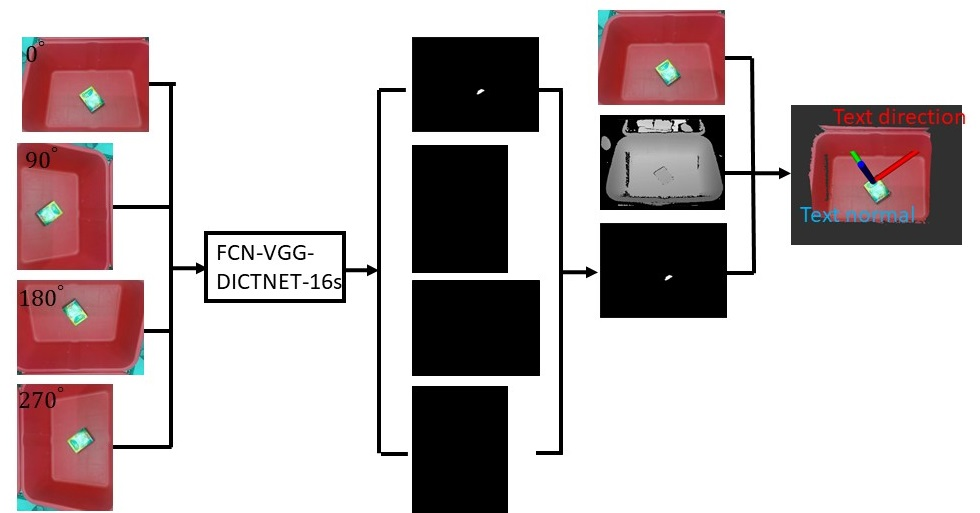
\includegraphics[height=!, width=1.0\linewidth, keepaspectratio=true]
	{./figures/text-pose-extimation-pipeline.jpg}
  \caption{基於品牌文字之語意切割與姿態預測流程圖}
  \label{figure:text-pose-extimation-pipeline}
\end{figure}

\paragraph{全卷積網路架構FCN-VGG-DICTNET}
此模型架構乃是利用卷積神經網路模型VGG-DICTNET ~\cite{jaderberg2014synthetic},並改成全卷積網路架構而成。VGG-DICTNET是一個文字分類模型,並以800,000張由電腦圖學方式所生成的文字圖片,可以用來分類88,172個字典出現過的文字。參考論文FCN~cite{long2015fully},透過將全連階層(fully connected layer)替換,改成全卷積層(fully convolutional layer)的方法,而得FCN-VGG-DICTNET。此模型輸入為灰階圖片,。而輸出則是一張有21個濃密標註的濃密積率地圖,並以圖片方式呈現。這21類包含20個類品牌文字類別與1類背景。

\subsection{夾取可行性預測}
\paragraph{2指假爪夾取可行性預測}
2指假爪夾取可行性預測乃基於品牌文字語意切割與姿態預測方法,分析品牌文字遮罩與姿態,本研究以遮罩大小進行排序,遮罩愈大可行性愈高,在考慮夾取姿態是否會受到盒子的阻礙進行排序,對預期會受到阻礙的夾取姿態濾除。


\paragraph{吸盤假爪夾取可行性預測}
吸盤假爪夾取可行性預測優先考慮品牌文字語意,在有看到品牌文字前提下,針對品牌文字遮罩進行吸取。若無品牌文字,則進行物品語意分析,對物品遮罩進行吸取。最後考量吸盤的特性,針對遮罩進行點雲分析進行可行性預測。受於吸盤假爪限制,吸盤只能從上而下垂直去吸取物品,而且吸盤適合以垂直平面方式去吸取,且不適合吸邊角,因此遮罩平面必須與吸盤垂直或大於80$^{\circ}$,且吸取點曲率也需低於一定門檻值。



\section{主動式操作系統}
在典型的夾取放置任務中,遮蔽與雜亂環境是造成失敗案例的主要原因,本研究所使用的基於品牌文字的方法當遇到遮蔽問題時,也無法解決。本研究在實驗中對於~\cite{peterthesis}提出的基於品牌文字之單手臂特定姿勢放置演算法,進行評估,證實其演算法在無遮蔽、雜亂場景下,可以有很高的成功率。但在雜亂場景中,如多個物品緊靠在一起、品牌文字朝下看不見的情況下,便會失敗。因此本研究提出兩階段主動式操作系統,去克服物體還有品牌文字被其餘物體遮蔽會失敗的問題,這個方法同時也能有效處理但品牌文字朝下,必須進行翻轉才能看到的問題。

\subsection{Baseline: 雙指假爪夾取與放置}
本研究所想進行比較的方法為雙指假爪夾取與放置演算法,當物體在不雜亂的環境中,而且品牌文字是可視的,這個方法可以有效執行特定姿勢放置任務。透過具旋轉差異性的品牌文字語意分割的方法,品牌文字姿態可以被有效預測,此外這個方法也假設藉由已知的物品模型,可以從品牌文字姿態推理得到夾取姿態。


\subsection{Proposed Method: 主動式操作系統}
本系統將Baseline進行有效分析,找出其缺點,並提出兩階段式主動式操作方法,改善對物品與品牌文字的感知能力及於雜亂空間中難以進行特定姿態夾取的問題。此系統乃根據基於品牌文字與物品幾何之夾取可行性預測演算法進行決策,決策方法為一個有限狀態機(Finite State Machine),並可根據觀察場景結果而分成兩類(可參考圖~\ref{figure:active_manipulation_and_baseline}):品牌文字可視與品牌文字不可視情況。

\begin{figure}[ht]
	\centering
	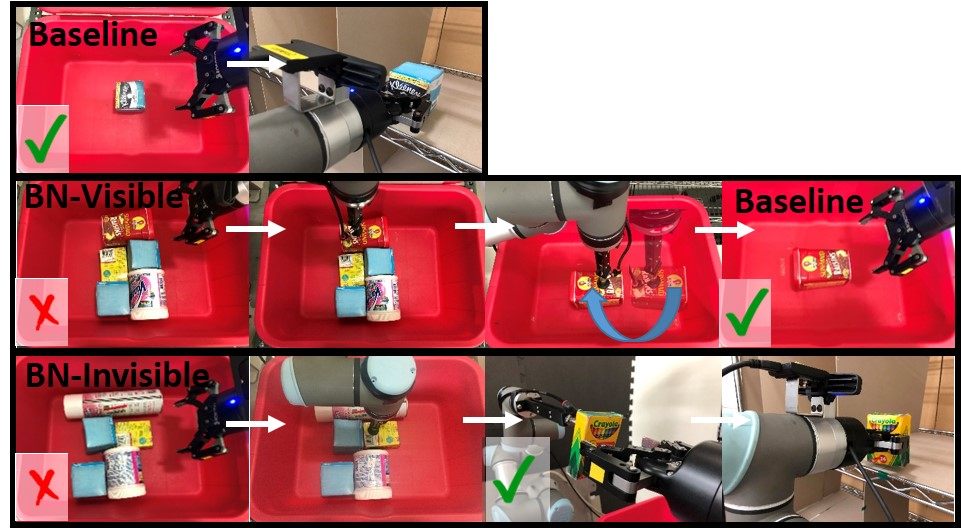
\includegraphics[height=!, width=1.0\linewidth, keepaspectratio=true]
	{./figures/active_manipulation_and_baseline.jpg}
  \caption{baseline與本研究所提出之主動式操作系統的連續行為。(第一排)在空曠環境中,且品牌文字可視的情況下,以baseline方法用特定姿態夾取物體。(第二排)在雜亂盒內,且品牌文字可視情況下,依序以吸盤假爪夾取物品、放置於乾淨盒子並擺正、以特定姿態夾取並放置架上。(第三排))在雜亂盒內,且品牌文字都不可視情況下,依序以吸盤假爪夾取物品、停留於空中並旋轉直至找到品牌文字、以特定姿態夾取並放置架上。
	}
  \label{figure:active_manipulation_and_baseline}
\end{figure}

\paragraph{品牌文字可視的狀況下}
在品牌文字可視的情況下,採取的策略為先使用吸盤假爪夾取放置到空曠盒子,再使用雙指假爪在空曠盒內以特定姿態夾取物體並放置到架上。採用如此的策略,是考量即使品牌文字可視,要在雜亂環境以特定姿態去夾取仍是一件困難的事情,因為夾取路徑可能會被其餘物品或盒子所阻礙。本研究搜尋之前於Amazon Picking Challenge的成果,大多隊伍都證明吸盤假爪在夾取的任務中,比雙指假爪效果好上許多,因此本研究基於吸盤假爪夾取可行性預測,找出物體品牌文字可吸區域,再用吸盤假爪從雜亂盒子夾取物品至乾淨盒子中央的策略。這有助於第二次的特定姿態夾取,也可使品牌文字置中,助於預測。此外,第一次夾取與放置行為中也包含把物體旋轉與水平線平行,讓品牌文字易於預測。而第二次的夾取放置任務則是採用baseline的方法。

\paragraph{品牌文字不可視的狀況下}
在品牌文字不可視的情況下,可預期品牌文字不在物體朝上的平面,因此採取的策略為使用吸盤假爪舉起物品至空中停留,並藉由旋轉物體的方法來找到品牌文字所在的那個平面。之後第二次的夾取,在看的到品牌文字的情況下,利用baseline方法,在空中以特定姿勢去夾取物品並放置。在第一次的夾取,乃利用物品語意分析的吸盤假爪夾取可行性預測,運用物體級別的全卷積網路影像切割,並利用點雲的法向量與曲率去找出適合夾取的點去進行夾取。

\subsection{主動式操作系統實作細節:有限狀態機}

主動式操作系統乃使用有限狀態機實現,每一個節點皆代表一個狀態與行為,綠色部份為手臂操作行為,而黑色部份則為深度攝影機進行夾取可行性評估行為。藉由將夾取可行性結果進行分類,以及狀態之間的轉移,系統可有效率的處理所有會遇到的狀況,完成可以應付遮蔽與雜亂環境的系統。

\paragraph{基於品牌文字之吸盤假爪夾取可行性評估 (物體於雜亂盒中}
在這一狀態,透過於雜亂盒子上方的深度攝影機觀察,進行基於品牌文字之吸盤夾爪夾取可行性評估,分析在場景中是否存在品牌文字,若有則對品牌文字進行語意分析,若無則轉換至``Suction area detection’’對物品進行基於物品語意之吸盤假爪夾取可行性語意分析。

\paragraph{基於物品語意之吸盤假爪夾取可行性評估 (物體於雜亂盒中)}

在看不見品牌文字的情況下,本研究進行基於物品語意之吸盤夾爪夾取可行性評估,
藉由VGG16-FCN進行物體切割。並結合點雲分析,找出物體適合夾取點。

\paragraph{夾取物品至空盒}
此狀態進行將單一個品牌文字可視的物體夾取至空盒中,並旋轉物品直至品牌文字與水平線平行。讓第2階段的感知與操作降低困難度。

\paragraph{夾取物品停留於空中並旋轉}
為驗證主動式操作可解決遮蔽,假設品牌文字於商品朝下平面,因此吸盤假爪夾起物品後朝向機械手臂UR5,並旋轉,準備讓嵌於UR5上的深度攝影機進行觀察。

\paragraph{基於品牌文字之2指假爪夾取可行性評估 (物體於空盒中)}
在這一狀態,可視為在空曠、無遮蔽雜亂環境中對物品進行基於品牌文字之2指假爪夾取可行性評估任務,預測出類別與特定姿勢夾取姿態。

\paragraph{基於品牌文字之2指假爪夾取可行性評估 (物體於UR3吸盤夾爪中}
此狀態執行的行為與前者相同,唯一不同的時,由於在前一狀態(夾取物品停留於空中並旋轉)夾取物品時,是依靠物品語意夾取,因此,並無法確定品牌文字的位置,因此無法保證於UR5的手臂能立即找出品牌文字,因此若無法找到品牌文字,則回到前一個階段,再次旋轉物體,若有預測出類別與特定姿勢夾取姿態。

\paragraph{夾取與放置到架上}
藉由從前一狀態所得夾取姿態及類別,2指假爪對物品執行夾取任務,並移動到上架準備位置,藉由Apriltag定位商品架,並將放置到指定格子,這些指定格子皆是人為定義於資料庫中。在任務執行完後手臂回到初始位置,繼續執行任務。


\begin{figure}[ht]
	\centering
	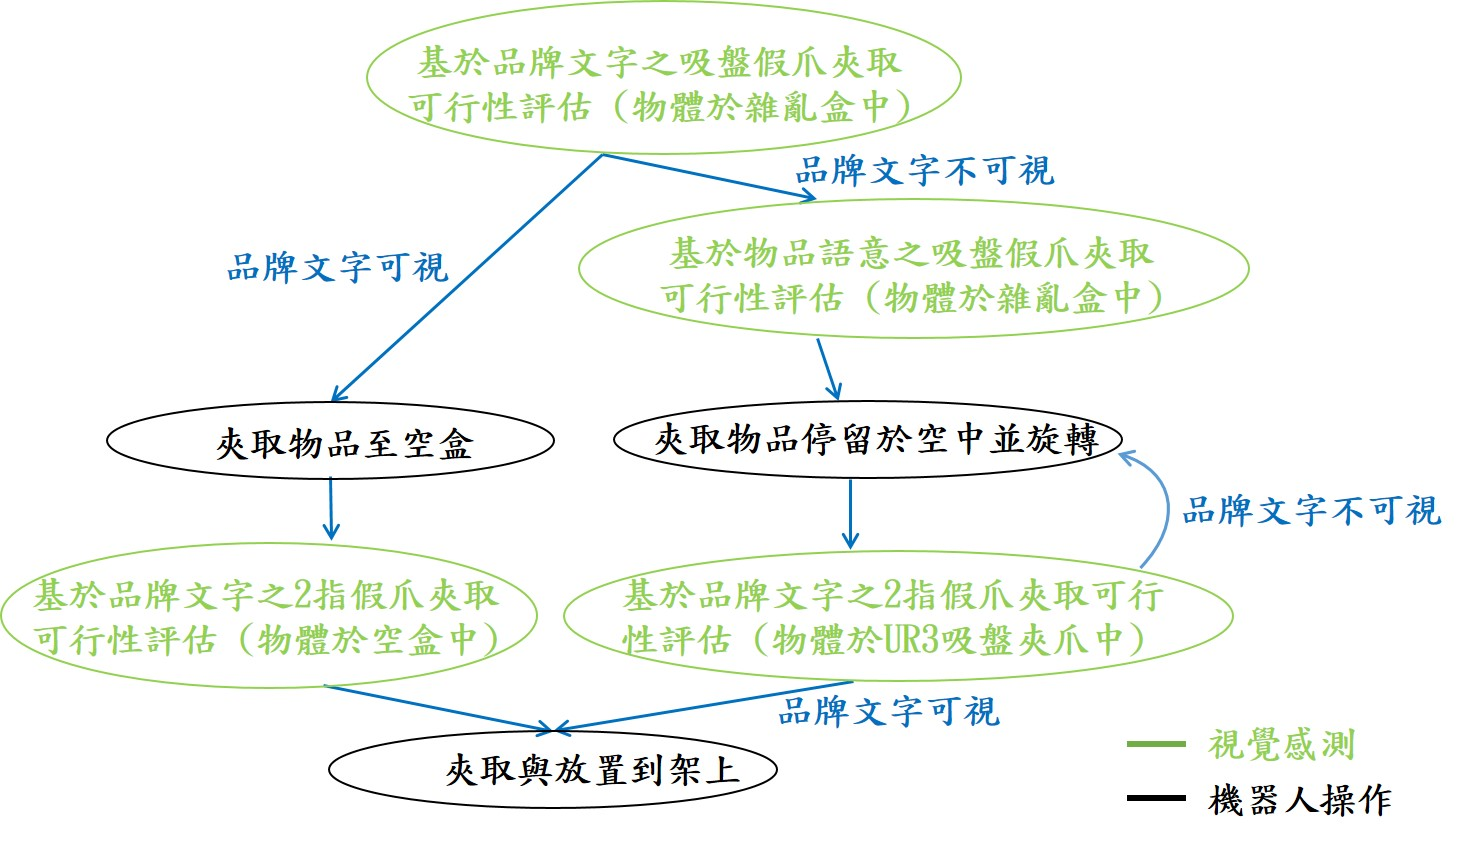
\includegraphics[height=!, width=1.0\linewidth, keepaspectratio=true]
	{./figures/FSM.jpg}
  \caption{主動式操作實作:有限狀態機}
  \label{figure:fsm}
\end{figure}
